\section{Bauformen von 3D Druckern}
Welche Arten von 3D Druckern gibt es ?
\subsection{Drucker nach Materialart}
\begin{itemize}
  \item \textbf{\uuline{SLA - Drucker}}
  \subitem \textbf{Stereolithografie}
  \subitem Erfinder: 1983  Chuck Hull
  \subitem Ebenfalls: STL-Schnittstelle
  \subitem (STereoLithography, Standard Tessellation Language)
  \item \textbf{\uuline{FDM - Drucker}}
  \subitem \textbf{Fused Deposition Modeling}
  \subitem 1985+ S. Scott Crump
  \subitem Auf Deutsch Schmelzschichtung
  \subitem Fused Filament Fabrication (FFF)
\end{itemize}


\newpage


\subsubsection{SLA - Stereolithografie - Drucker}

\begin{center}
  \vspace{-0.5cm}
  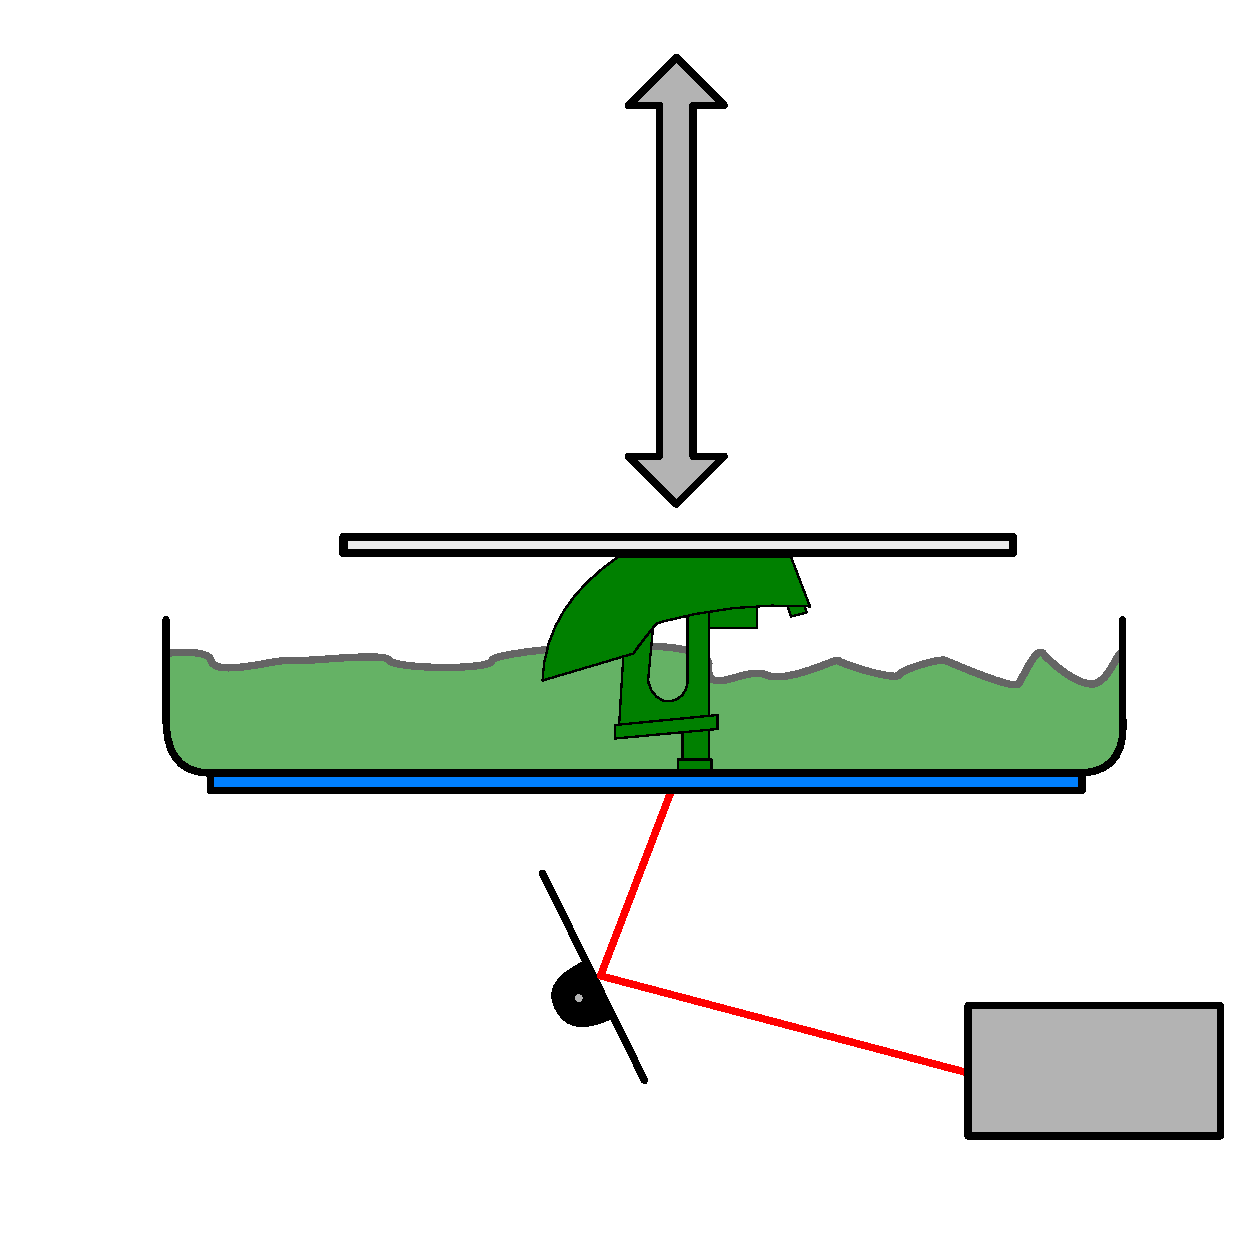
\includegraphics[width=0.6\textwidth, trim = 0px 45px 0px 10px, clip]{./bilder/SLA.pdf}
\end{center}

Verwenden Resin welches durch Licht ausgehärtet wird. \\
(Teuer. Kosten 80-100€ pro Liter.)


\newpage
\subsubsection{FDM (Fused Deposition Modeling) - Drucker}
\begin{center}
  \vspace{-1,7cm}
  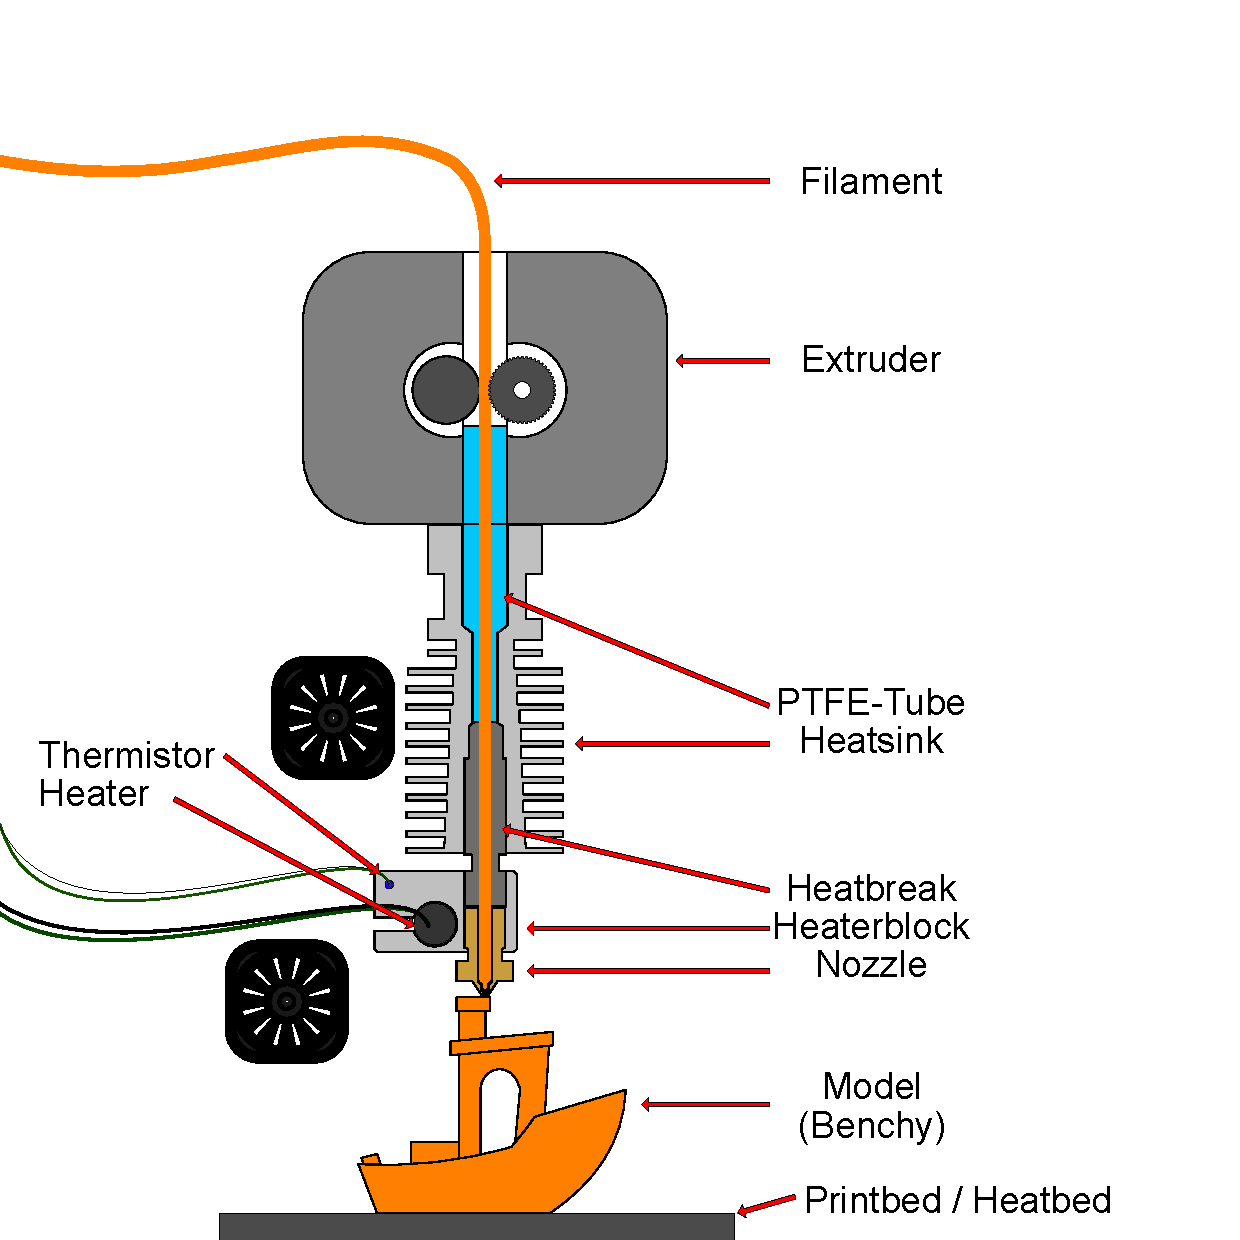
\includegraphics[width=0.6\textwidth]{./bilder/3dprinting.pdf}
\end{center}
Verwenden Filament auf Spulen.\\
(Kosten 13+ € pro Kilo / wobei gutes Filament bei 18€ anfängt)


\newpage % =
